\clearpage
\section*{Timing Diagrams}
Because the timing diagrams are so long, they are split across multiple screen shots.\\
However each row of the image is always the same signal.\\
From top to bottom, there are:
\begin{itemize}
    \item \verb+Clock+
    \item \verb+iCode+
    \item \verb+iFun+
    \item \verb+rA+
    \item \verb+rB+
    \item \verb+valC+
    \item \verb+valP+
    \item \verb+valA+
    \item \verb+valB+
    \item \verb+valE+
    \item \verb+valM+
    \item \verb+(new) PC+
\end{itemize}

\clearpage
\subsection*{Call Test}
\begin{figure}[!ht]
    \centering
    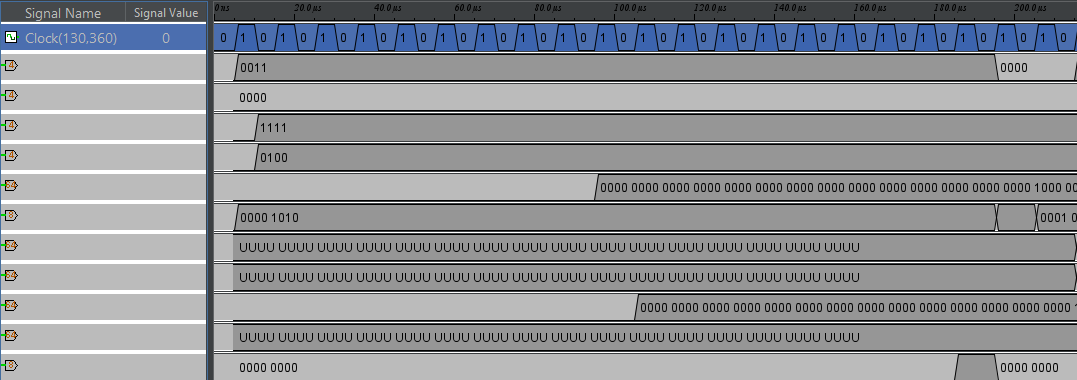
\includegraphics[width=\textwidth]{Images/Call Test Part 1.png}
    \caption{Call Test Part 1}
\end{figure}

\begin{figure}[!ht]
    \centering
    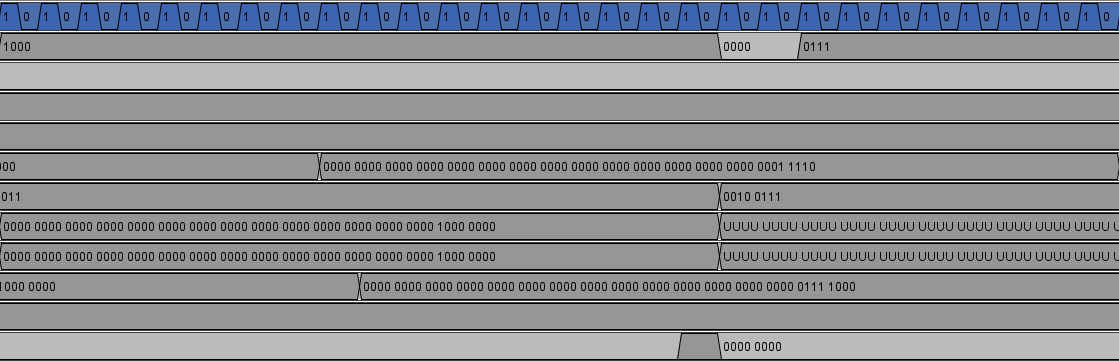
\includegraphics[width=\textwidth]{Images/Call Test Part 2.png}
    \caption{Call Test Part 2}
\end{figure}

\begin{figure}[!ht]
    \centering
    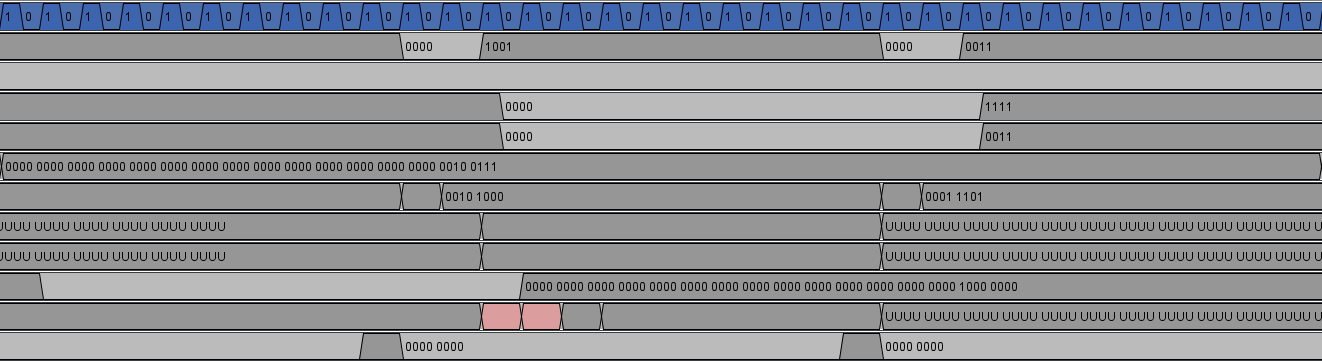
\includegraphics[width=\textwidth]{Images/Call Test Part 3.png}
    \caption{Call Test Part 3}
\end{figure}

\begin{figure}[!ht]
    \centering
    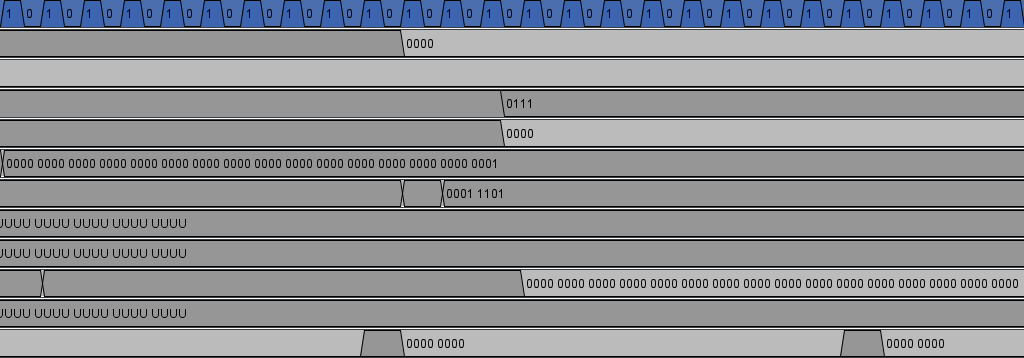
\includegraphics[width=\textwidth]{Images/Call Test Part 4.png}
    \caption{Call Test Part 4}
\end{figure}

\clearpage
\subsection*{OP Test}
\begin{figure}[!ht]
    \centering
    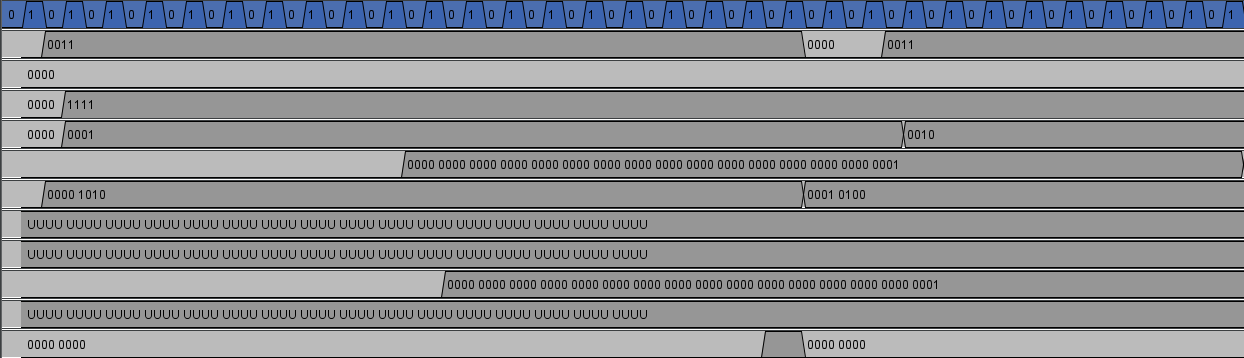
\includegraphics[width=\textwidth]{Images/OP Test Part 1.png}
    \caption{OP Test Part 1}
\end{figure}

\begin{figure}[!ht]
    \centering
    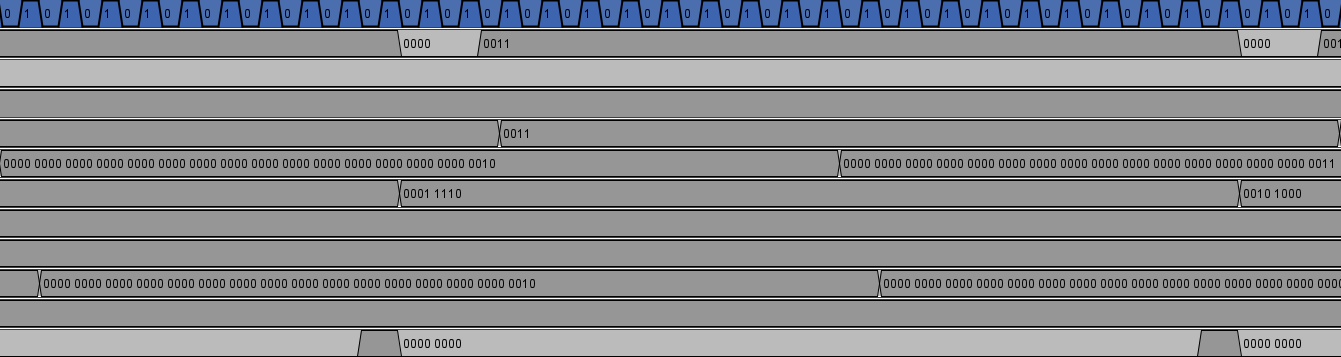
\includegraphics[width=\textwidth]{Images/OP Test Part 2.png}
    \caption{OP Test Part 2}
\end{figure}

\begin{figure}[!ht]
    \centering
    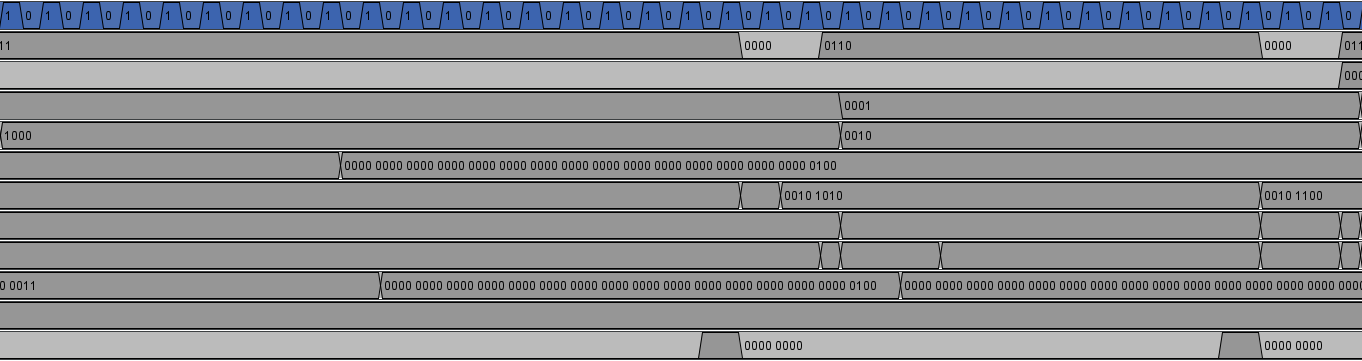
\includegraphics[width=\textwidth]{Images/OP Test Part 3.png}
    \caption{OP Test Part 3}
\end{figure}

\begin{figure}[!ht]
    \centering
    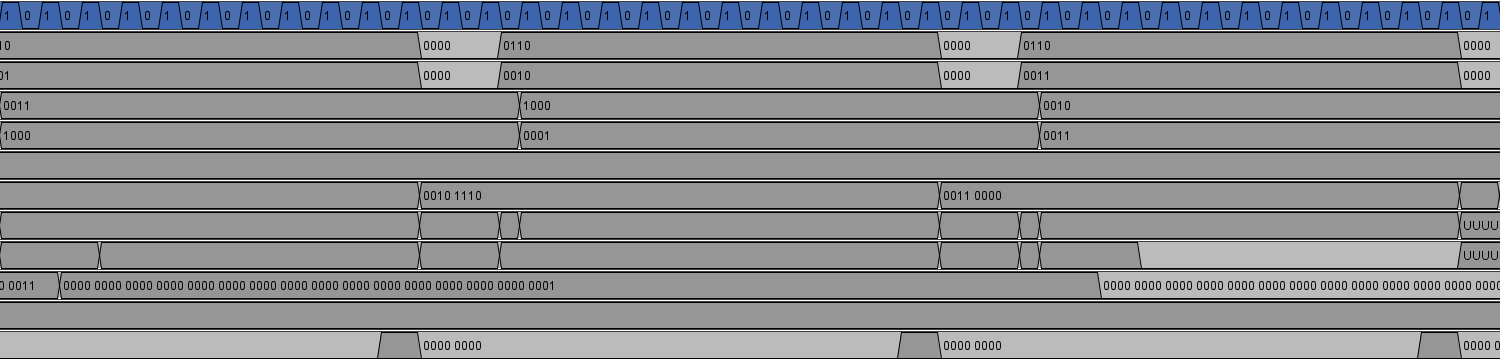
\includegraphics[width=\textwidth]{Images/OP Test Part 4.png}
    \caption{OP Test Part 4}
\end{figure}

\begin{figure}[!ht]
    \centering
    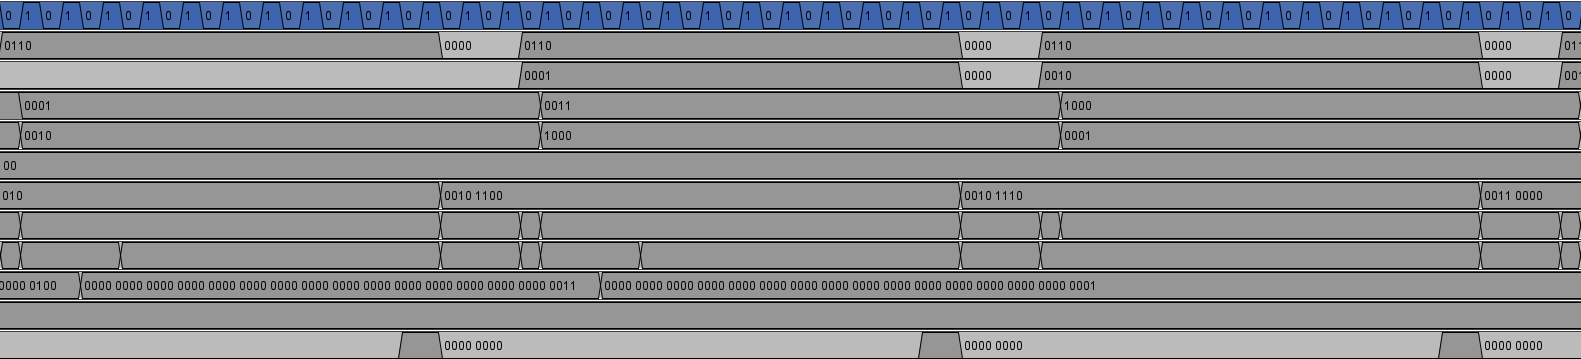
\includegraphics[width=\textwidth]{Images/OP Test Part 5.png}
    \caption{OP Test Part 5}
\end{figure}

\begin{figure}[!ht]
    \centering
    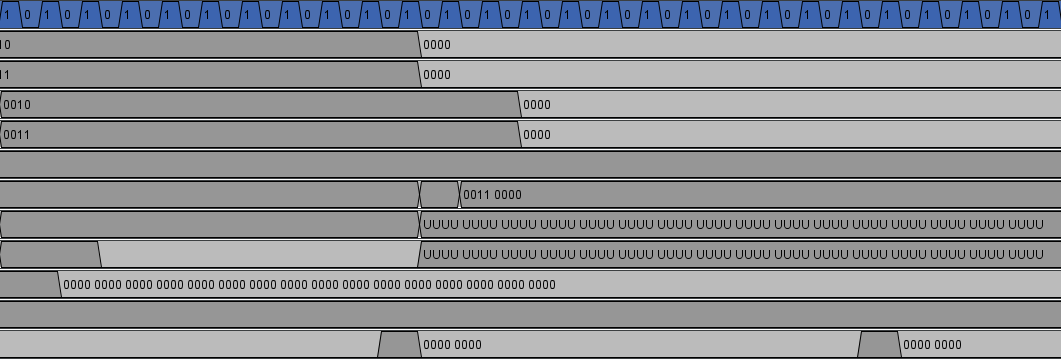
\includegraphics[width=\textwidth]{Images/OP Test Part 6.png}
    \caption{OP Test Part 6}
\end{figure}

\clearpage
\subsection*{Push Pop Test}
\begin{figure}[!ht]
    \centering
    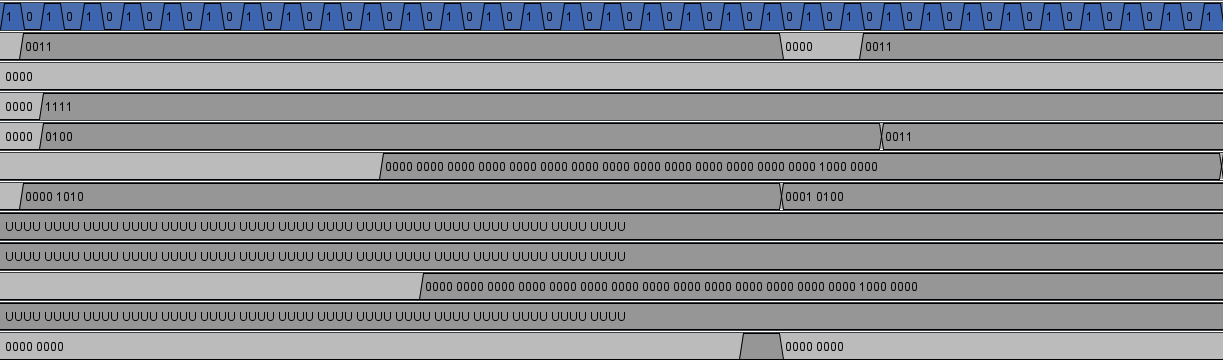
\includegraphics[width=\textwidth]{Images/PP Test Part 1.png}
    \caption{Push Pop Test Part 1}
\end{figure}

\begin{figure}[!ht]
    \centering
    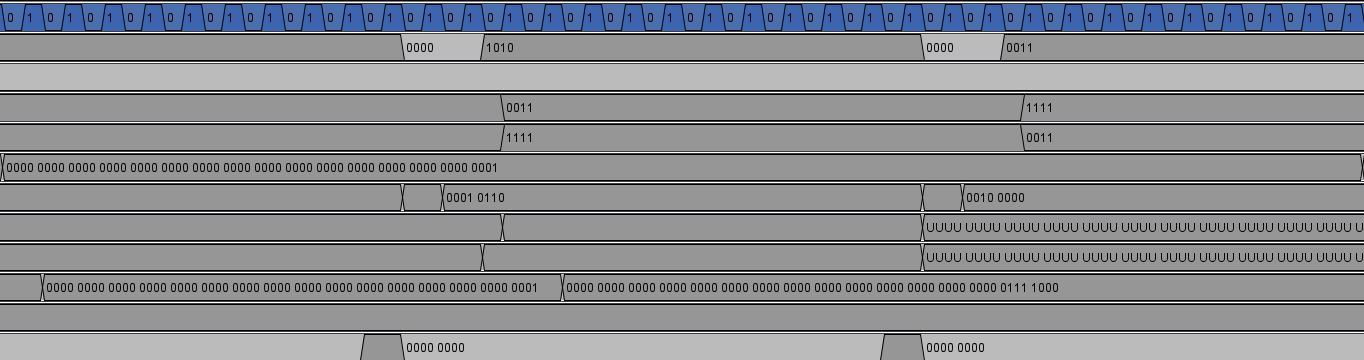
\includegraphics[width=\textwidth]{Images/PP Test Part 2.png}
    \caption{Push Pop Test Part 1}
\end{figure}

\begin{figure}[!ht]
    \centering
    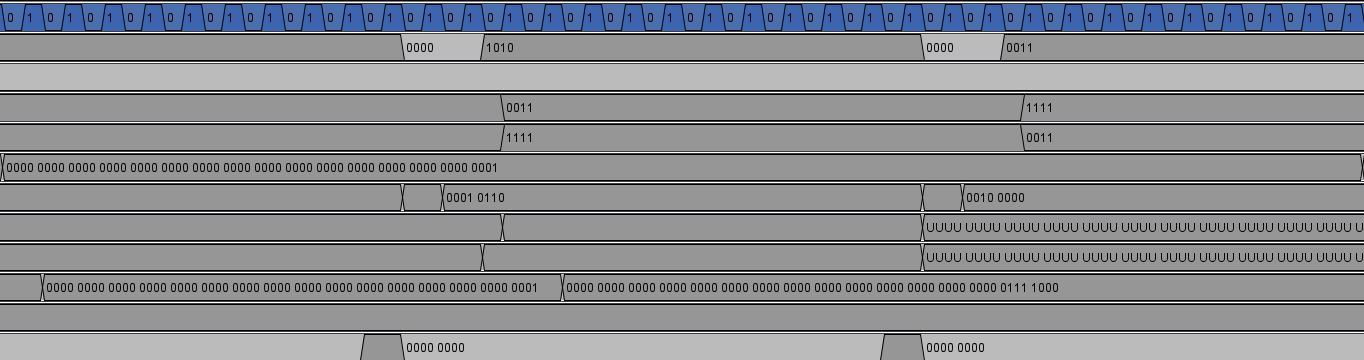
\includegraphics[width=\textwidth]{Images/PP Test Part 3.png}
    \caption{Push Pop Test Part 1}
\end{figure}

\clearpage
\subsection*{Register Test}
\begin{figure}[!ht]
    \centering
    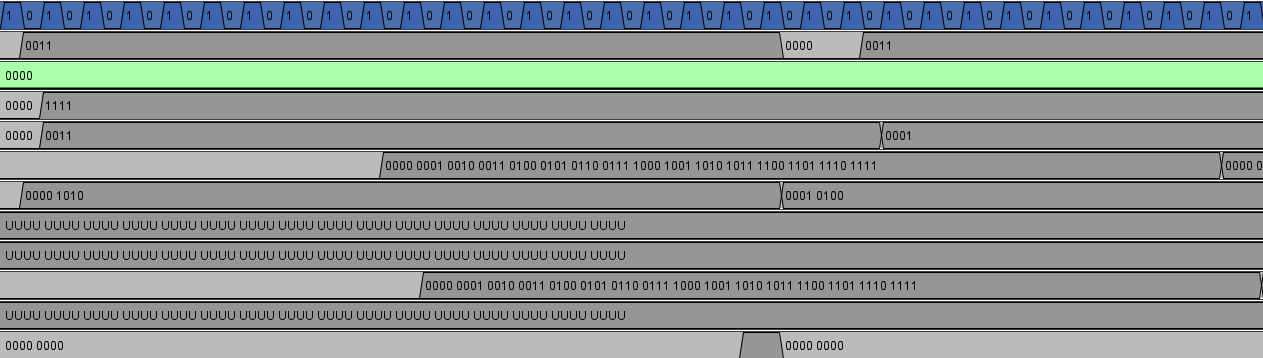
\includegraphics[width=\textwidth]{Images/Register Test Part 1.png}
    \caption{Register Test Part 1}
\end{figure}

\begin{figure}[!ht]
    \centering
    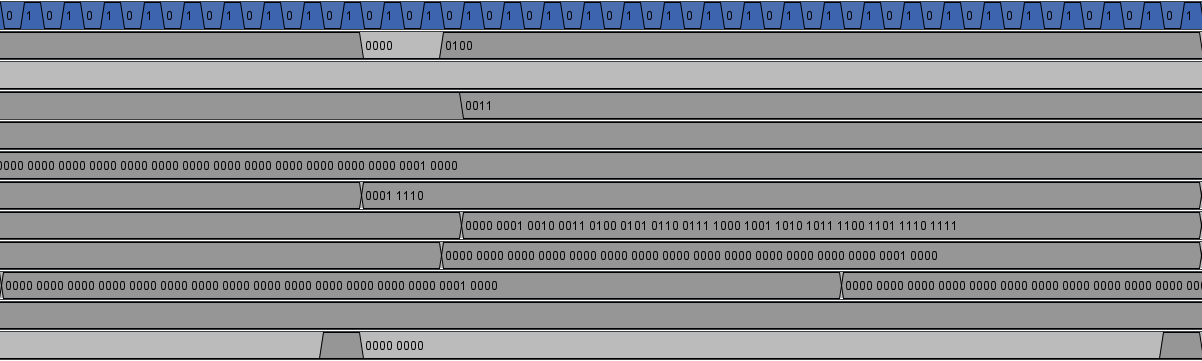
\includegraphics[width=\textwidth]{Images/Register Test Part 2.png}
    \caption{Register Test Part 2}
\end{figure}

\begin{figure}[!ht]
    \centering
    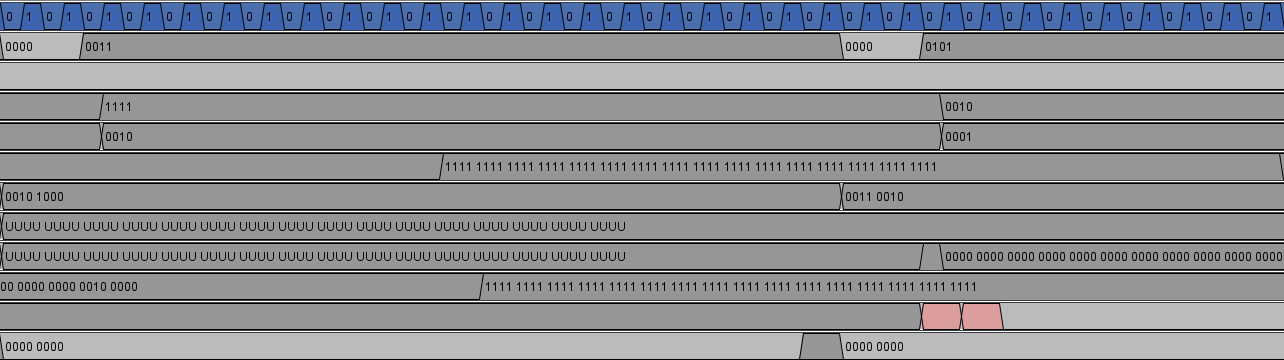
\includegraphics[width=\textwidth]{Images/Register Test Part 3.png}
    \caption{Register Test Part 3}
\end{figure}

\begin{figure}[!ht]
    \centering
    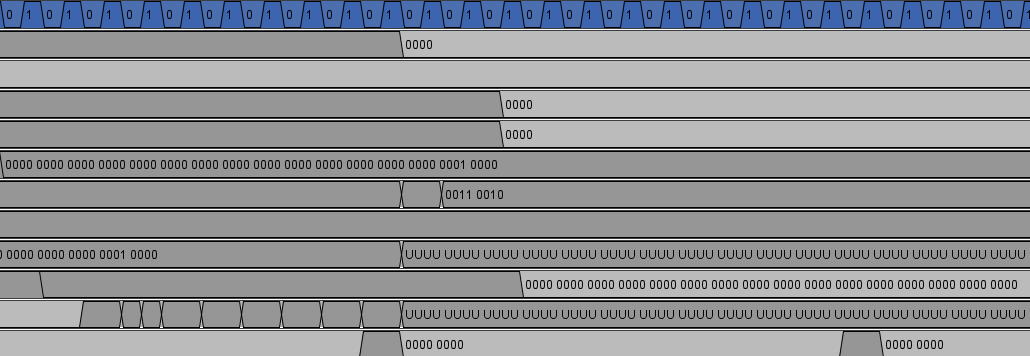
\includegraphics[width=\textwidth]{Images/Register Test Part 4.png}
    \caption{Register Test Part 4}
\end{figure}